% This file has to be locally compiled in terminal since no cite command is present

\documentclass[../main/thesis.tex]{subfiles}
\graphicspath{{thesis/appendix/figures/}}
% \graphicspath{{/home/arefk/uio/MScThesis_AreKvanum2022_SeaIceML/thesis/appendix/figures/}}

\begin{document}

\section{Code availability}
The code developed for this thesis is located in a GitHub repository in order to reproduce the analysis: \\
\url{https://github.com/AreFrode/MScThesis_AreKvanum2022_SeaIceML}.
For details regarding project structure or specifics about the code, refer to the README located in the GitHub-root.

\newpage

\section{Supporting Figures}

\begin{figure}[h]
    \centering
    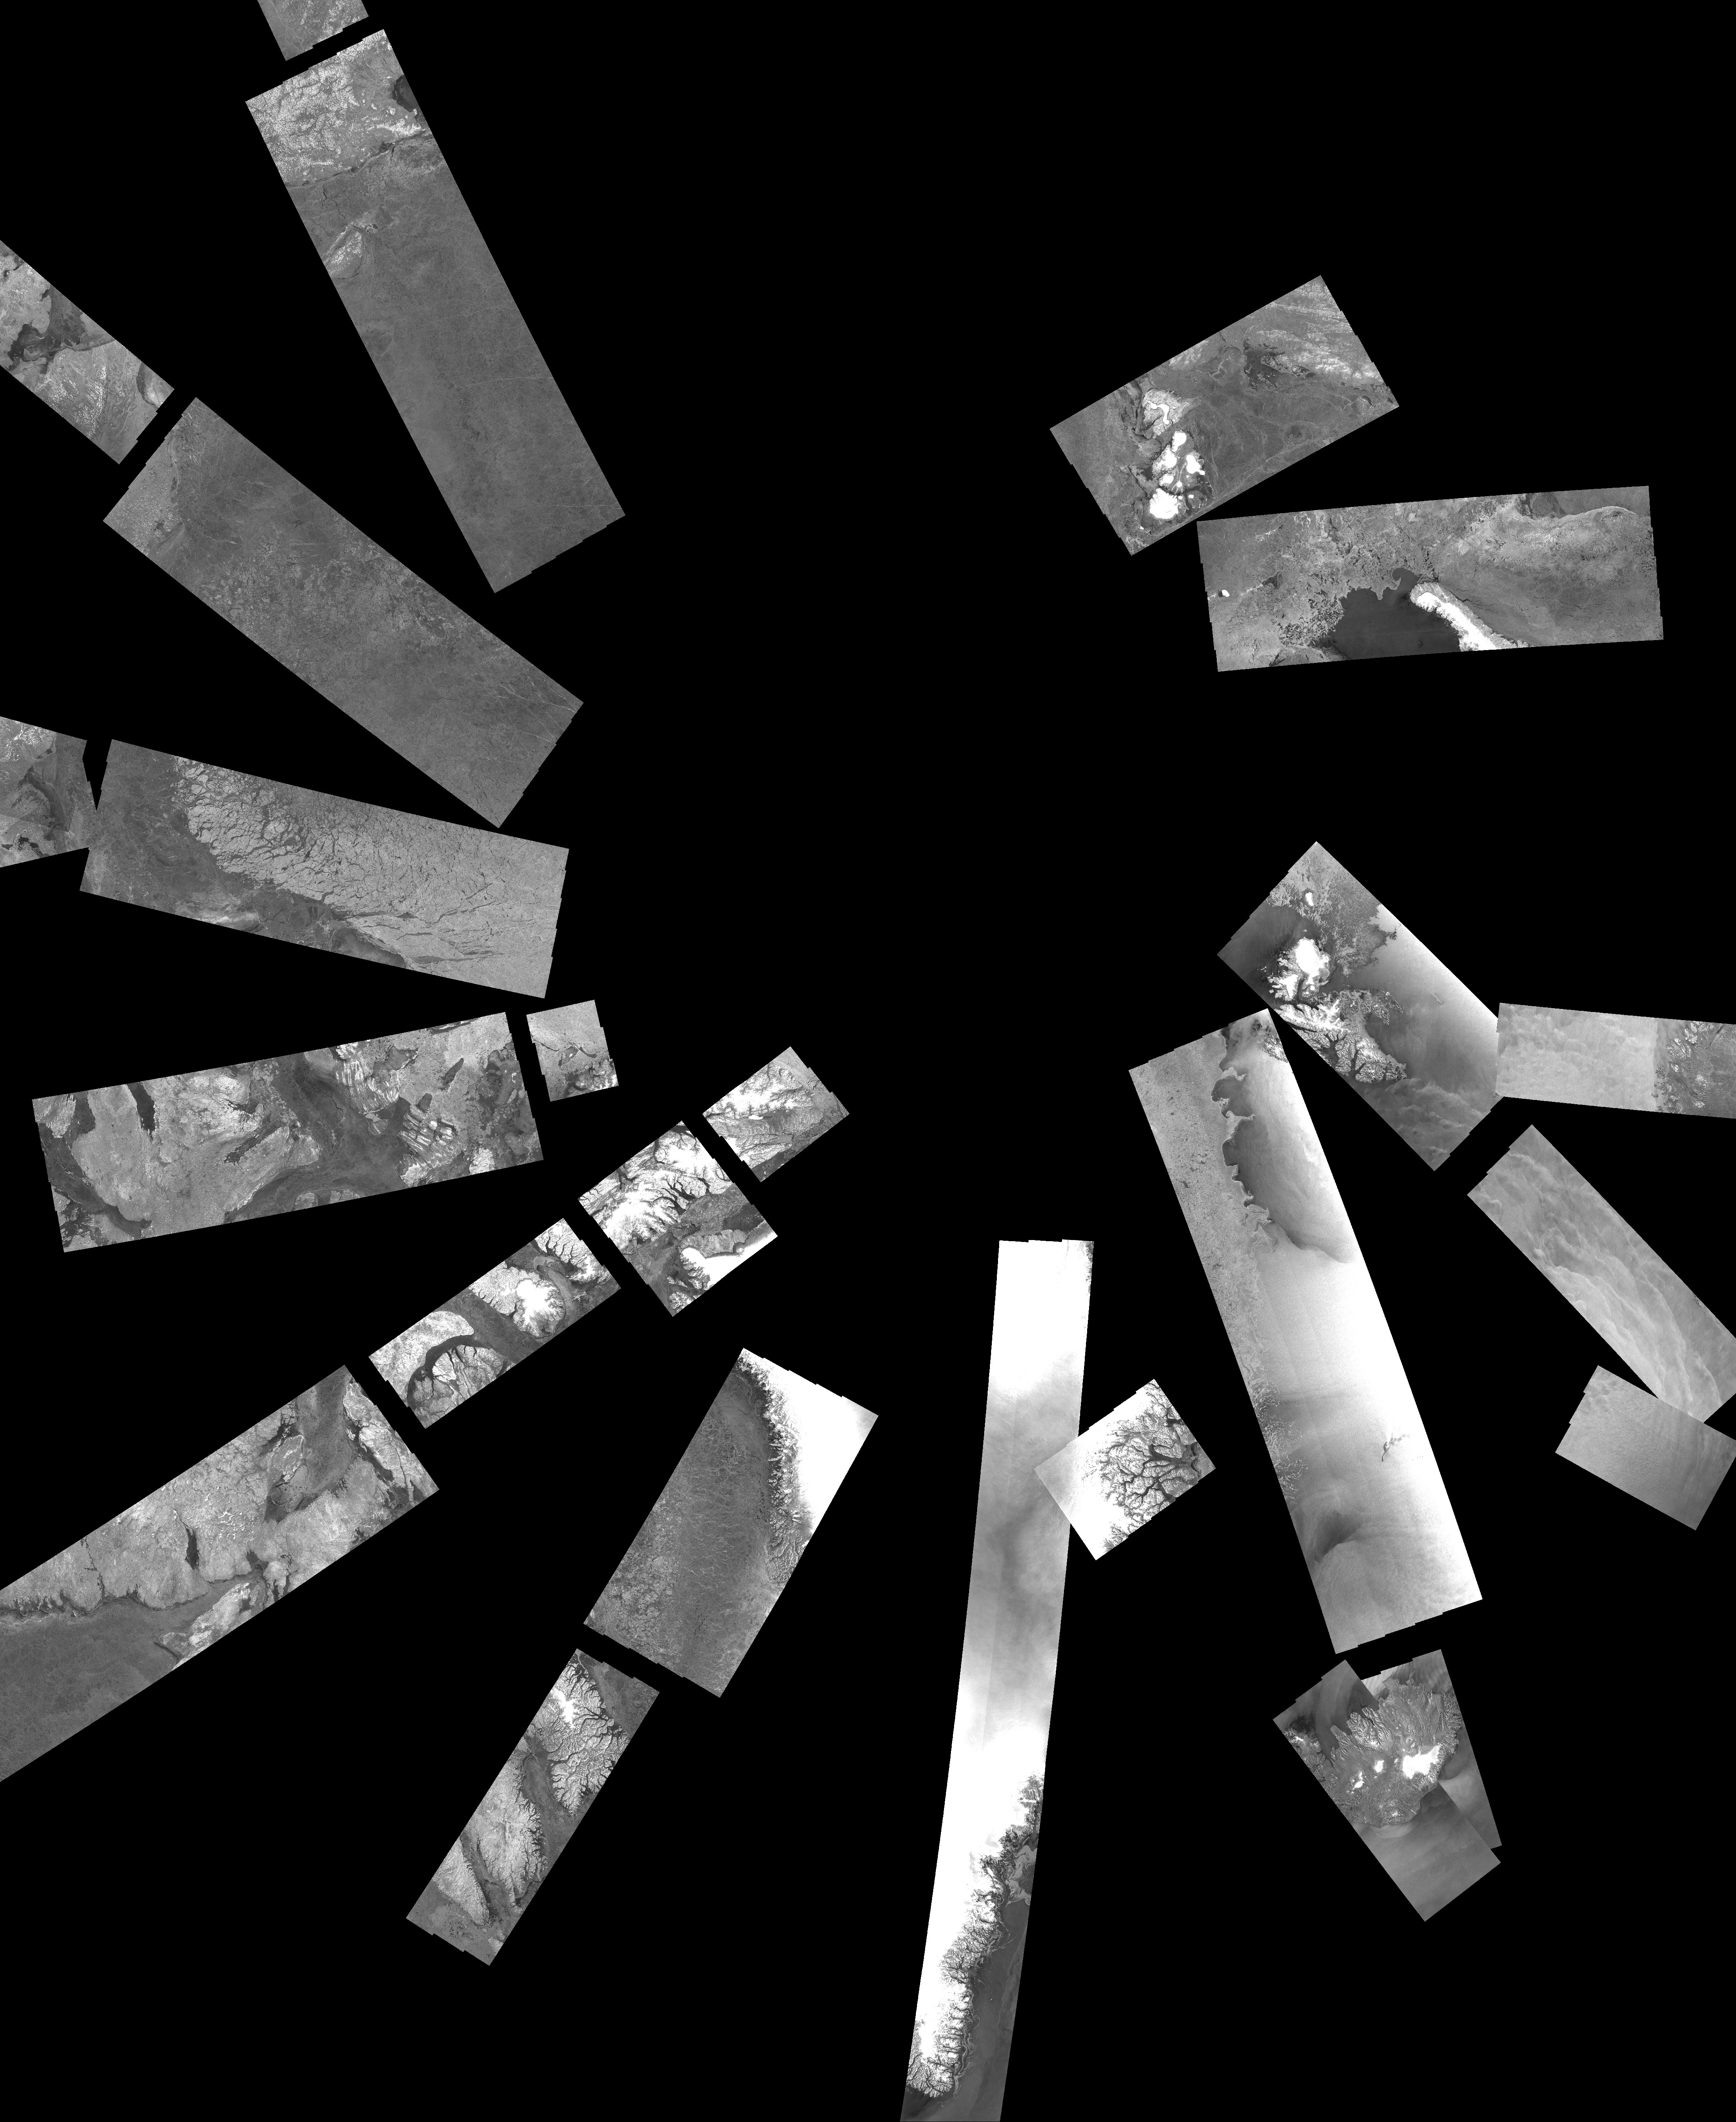
\includegraphics[width=0.725\textwidth]{dailysar}
    \caption{\label{fig:S-sar}Daily SAR observations of the Arctic from Sentinel 1A 23 Jan 2023}
\end{figure}

\begin{figure}
    \centering
    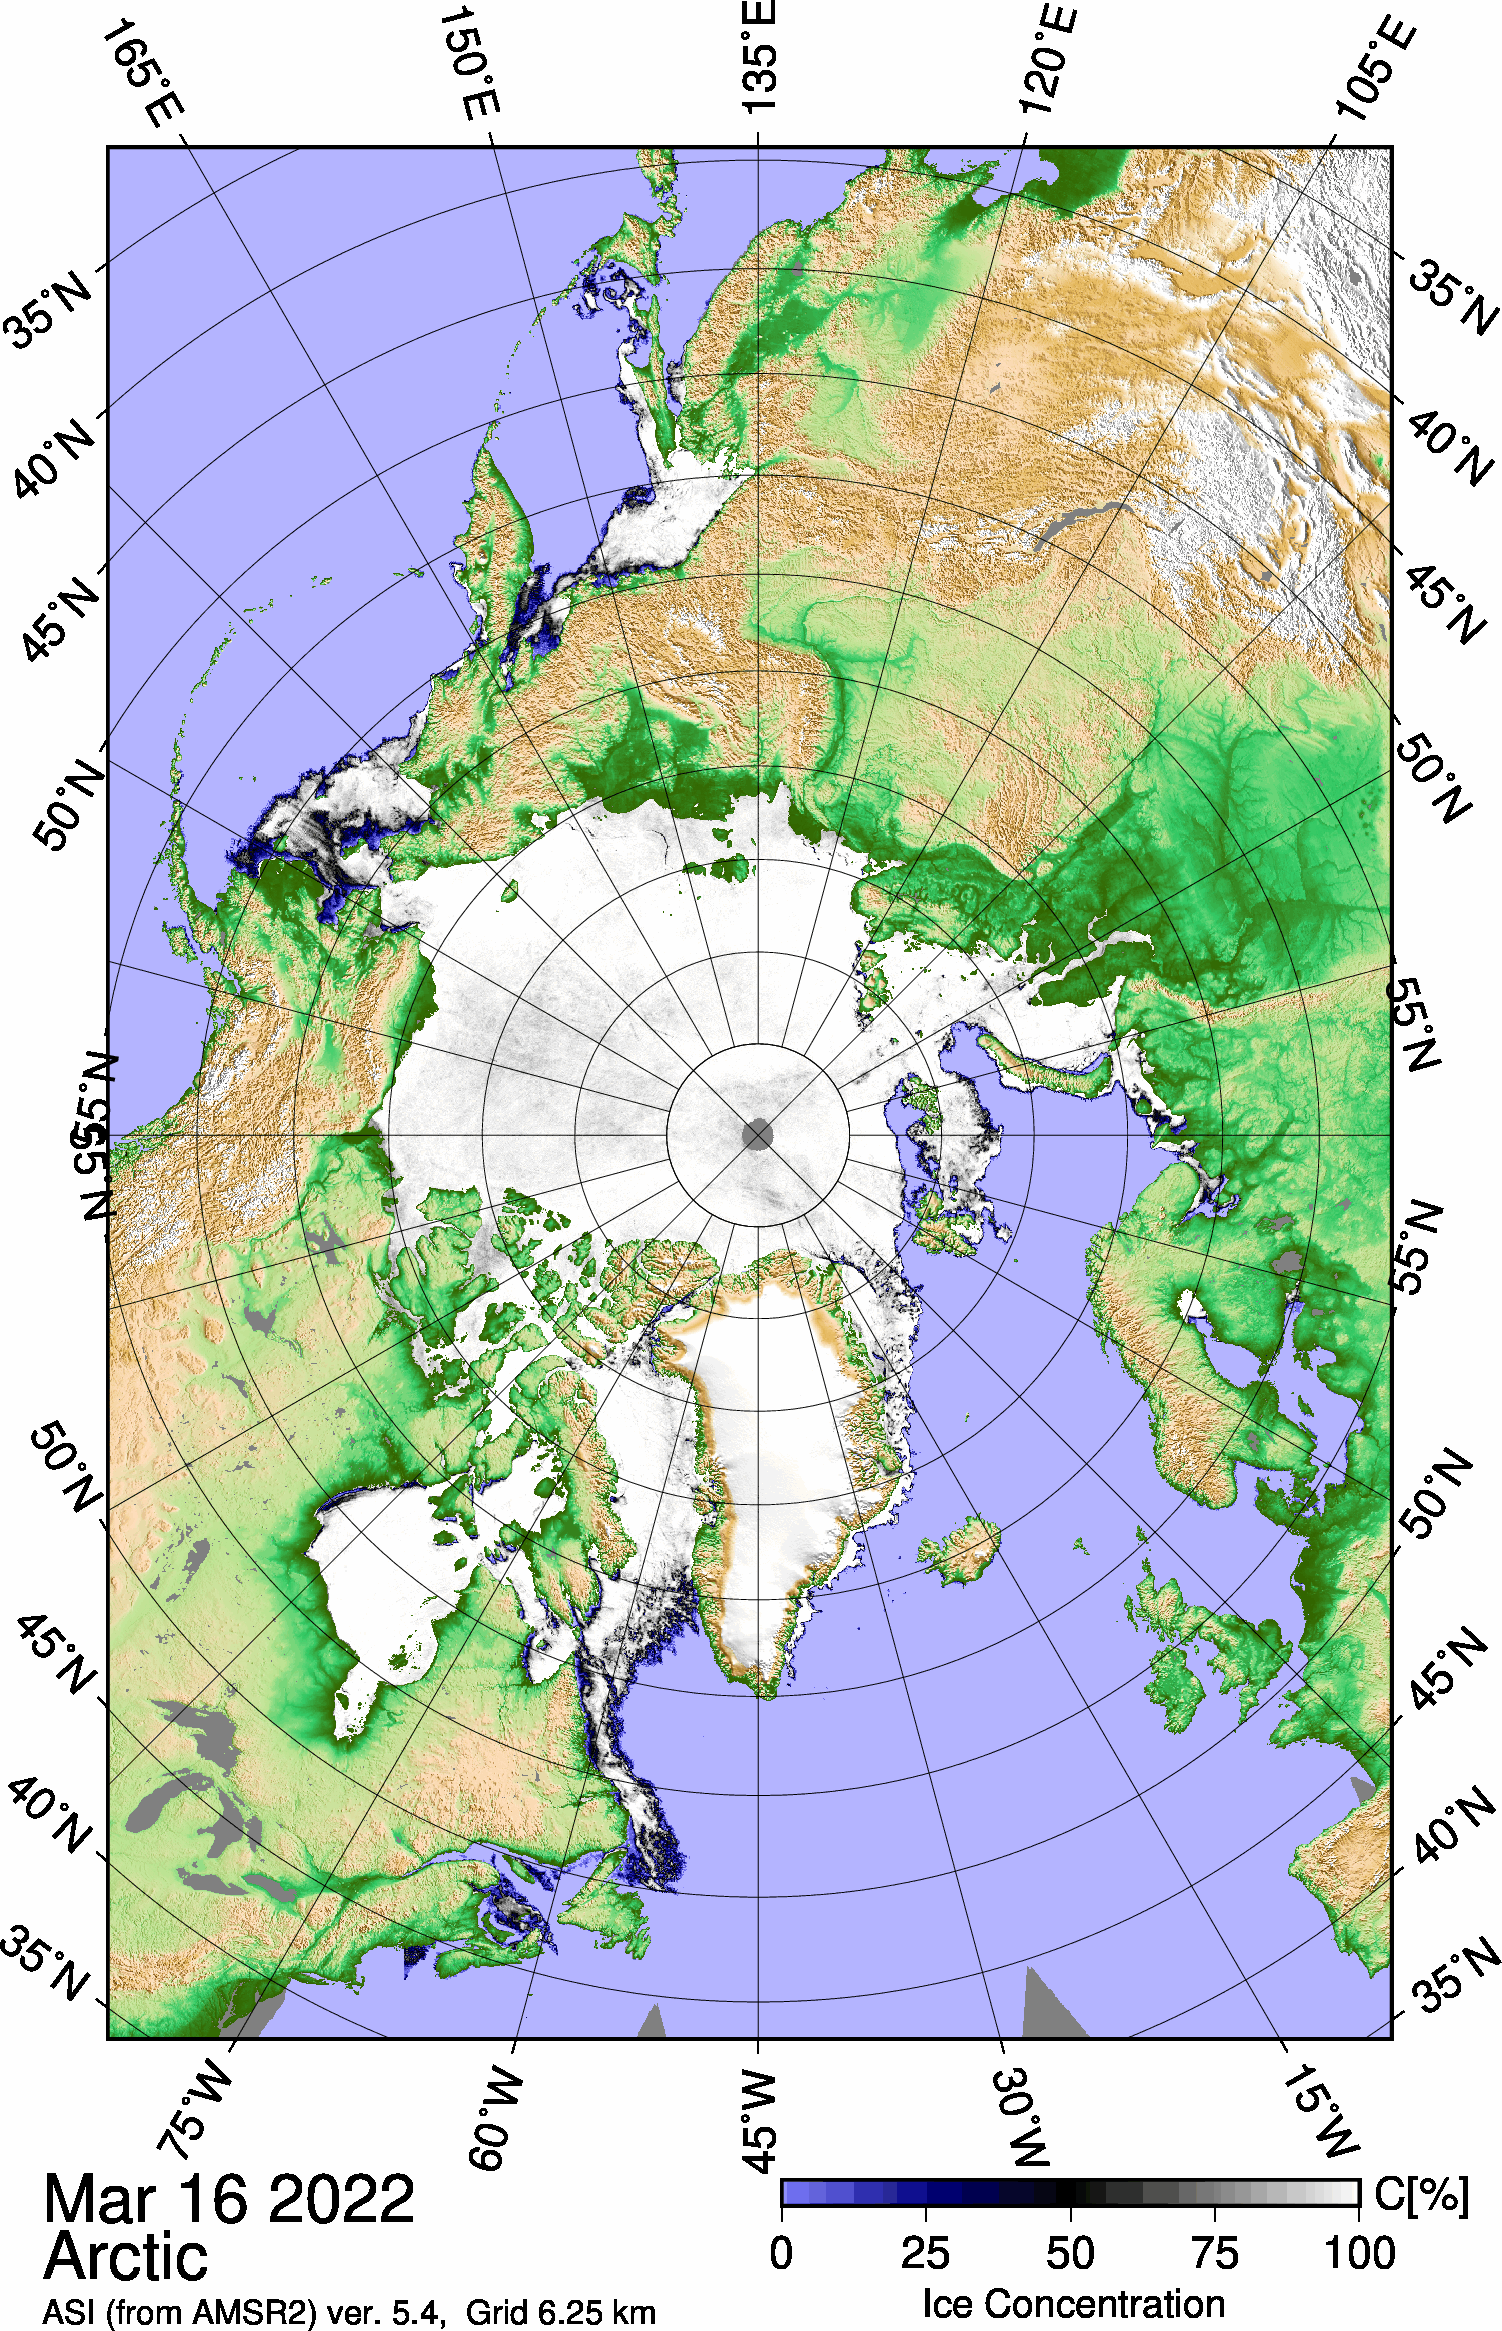
\includegraphics[width=.8\textwidth]{amsr216.png}
    \caption{\label{fig:S-amsr2-16}AMSR2 observations of the Arctic sea ice concentration 16 Mar 2022.}
\end{figure}

\begin{figure}
    \centering
    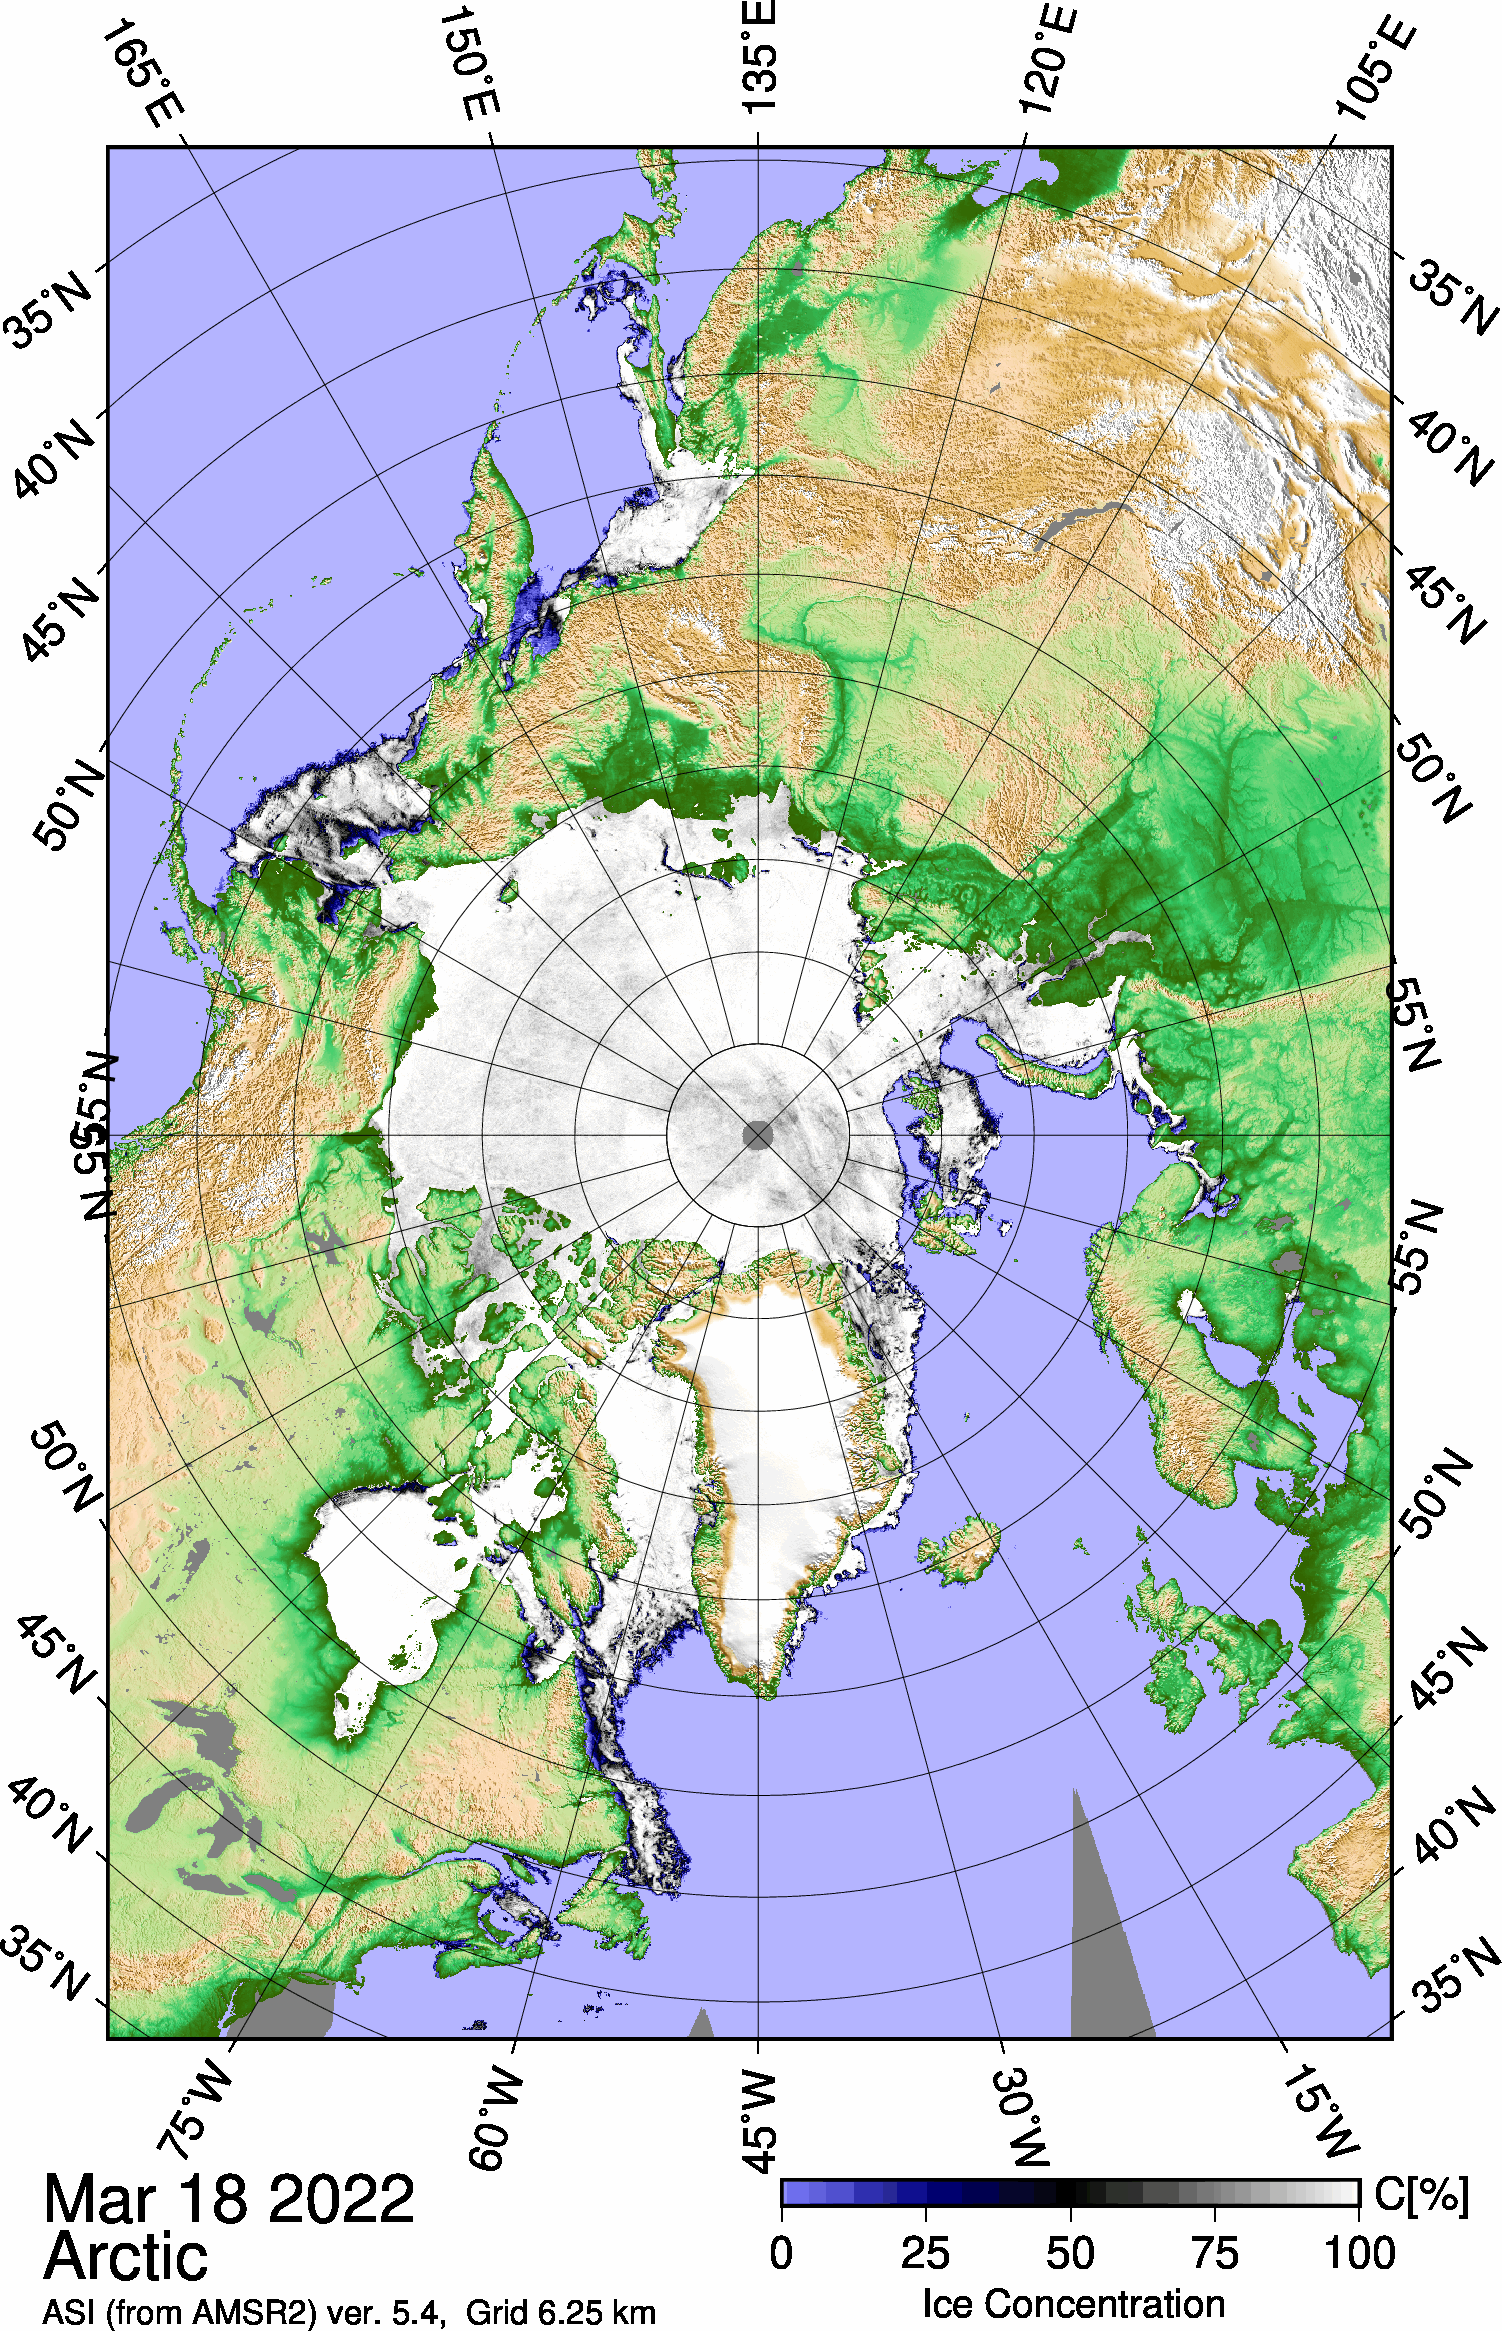
\includegraphics[width=.8\textwidth]{amsr218.png}
    \caption{\label{fig:S-amsr2-18}AMSR2 observations of the Arctic sea ice concentration 18 Mar 2022.}
\end{figure}

\newpage

\section{Poster contribution to The 11th International Workshop on Sea Ice Modelling, Assimilation, Observations, Predictions and Verification}

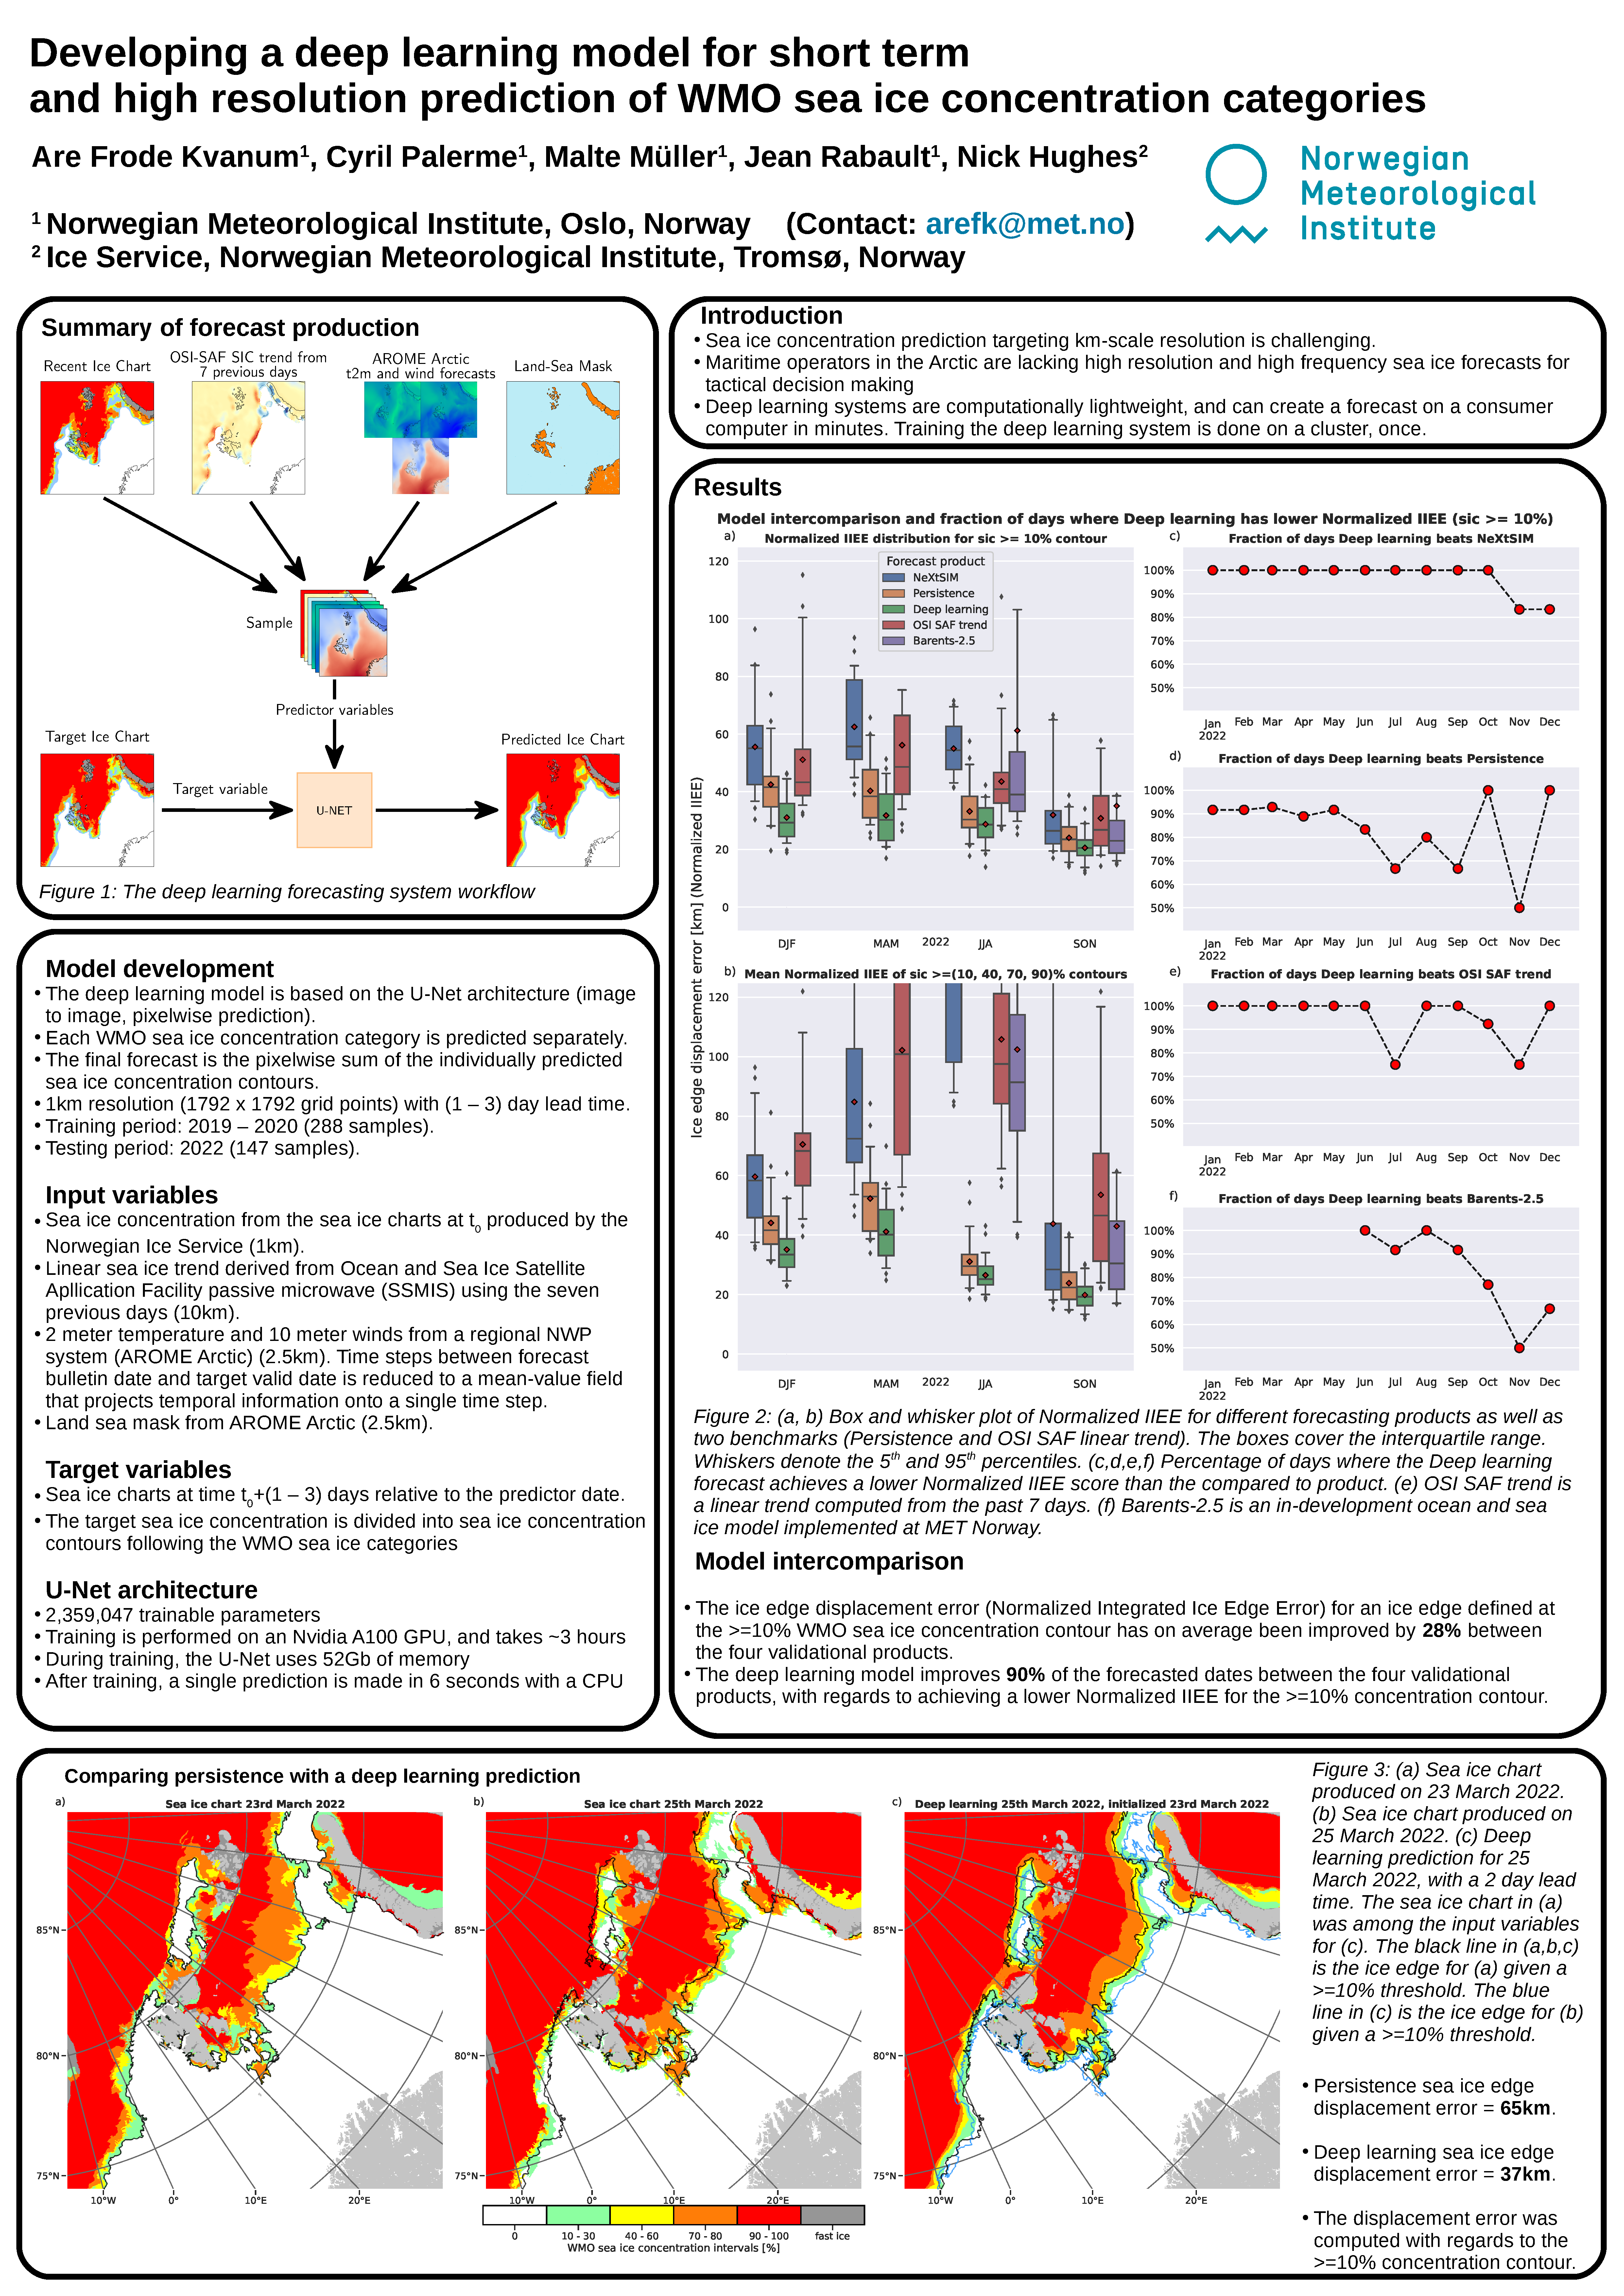
\includepdf{../appendix/figures/poster_final.pdf}

\end{document}